\begin{figure}[htp]
  \centering
  \subfloat[Naive approach]{\label{figur:1}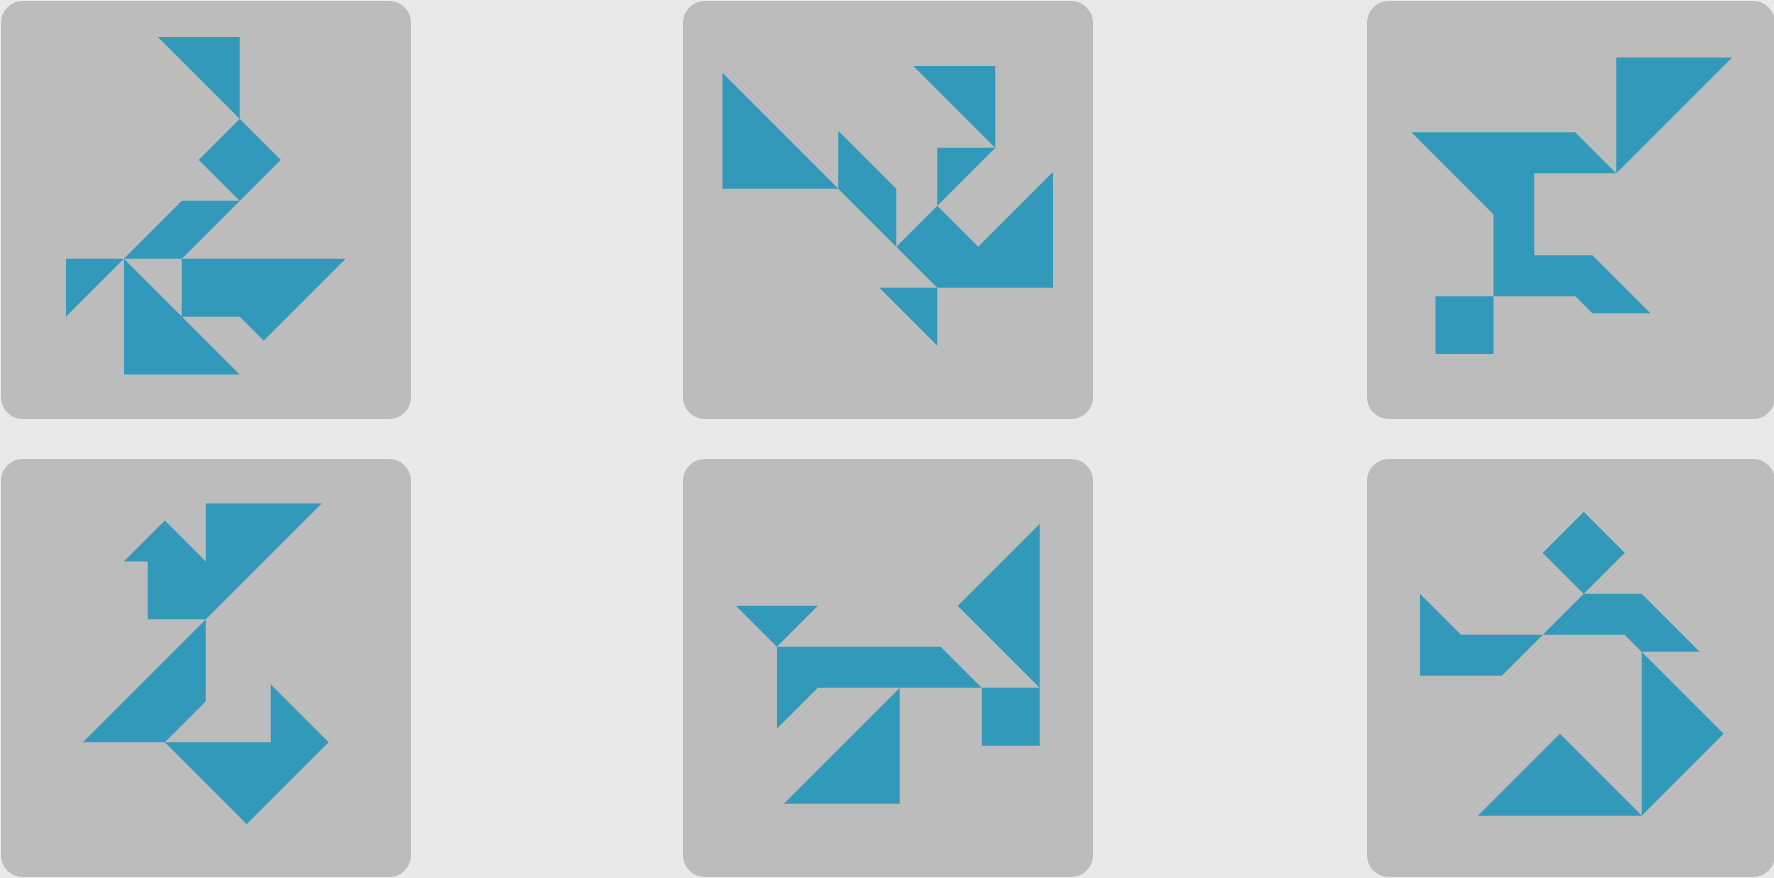
\includegraphics[width=0.45\textwidth]{figures/gen.png}}
  \hfill
  \subfloat[Naive approach with lower range threshold]{\label{figur:2}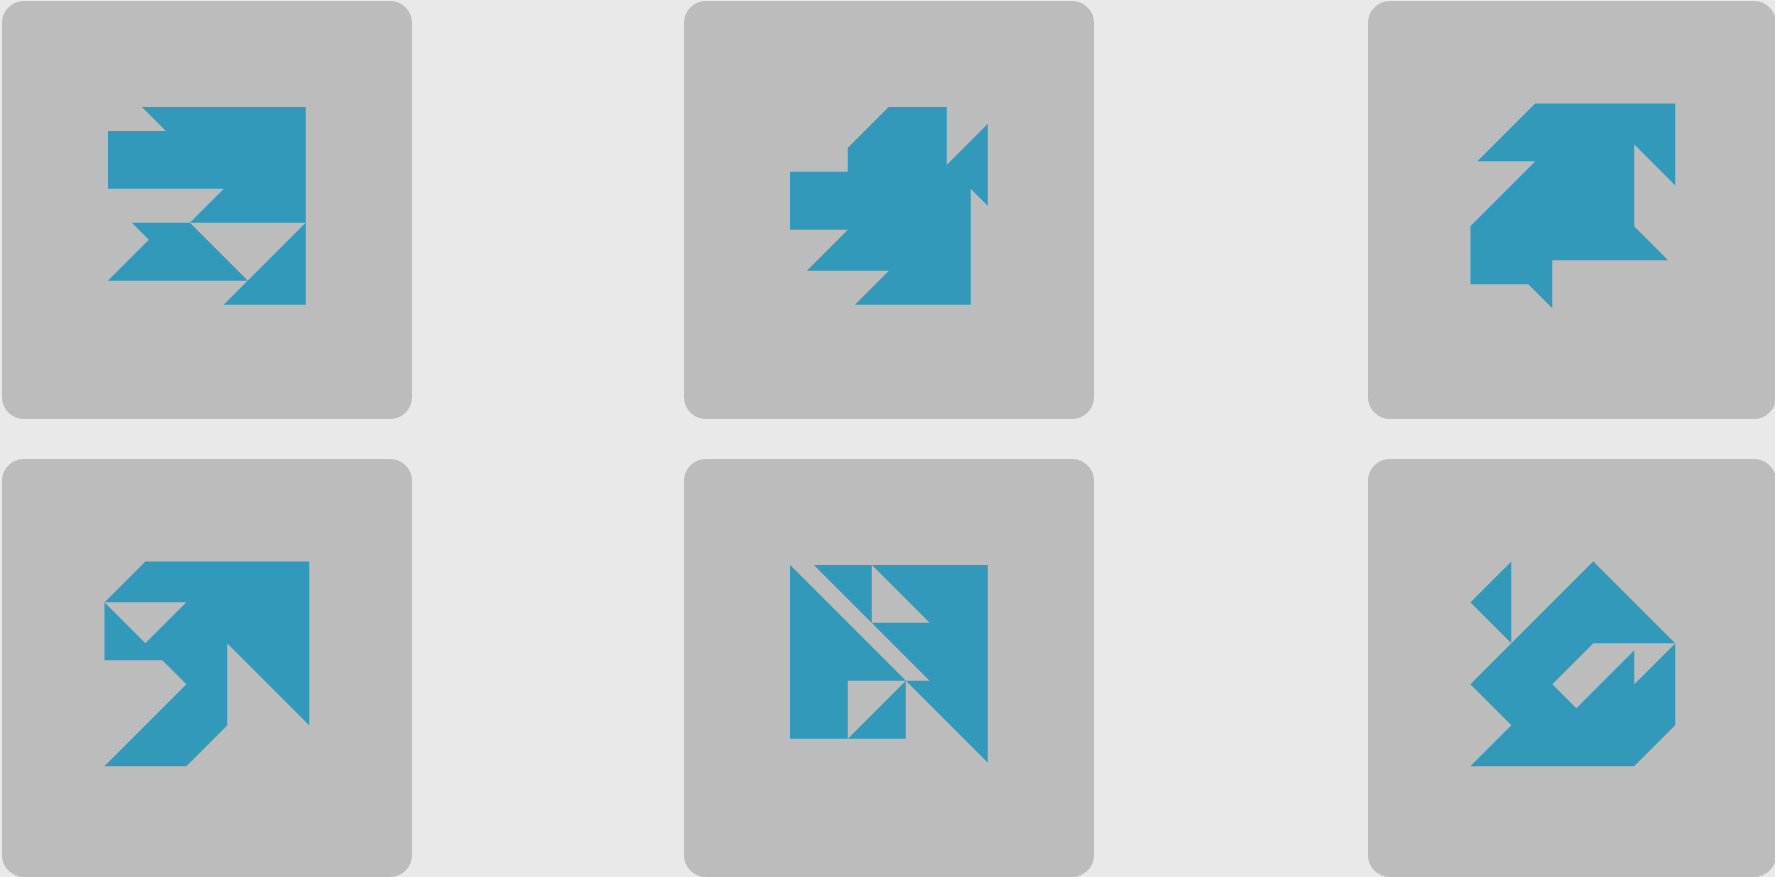
\includegraphics[width=0.45\textwidth]{figures/genSR.png}}
  \\
  \subfloat[Edge-matching approach]{\label{figur:3}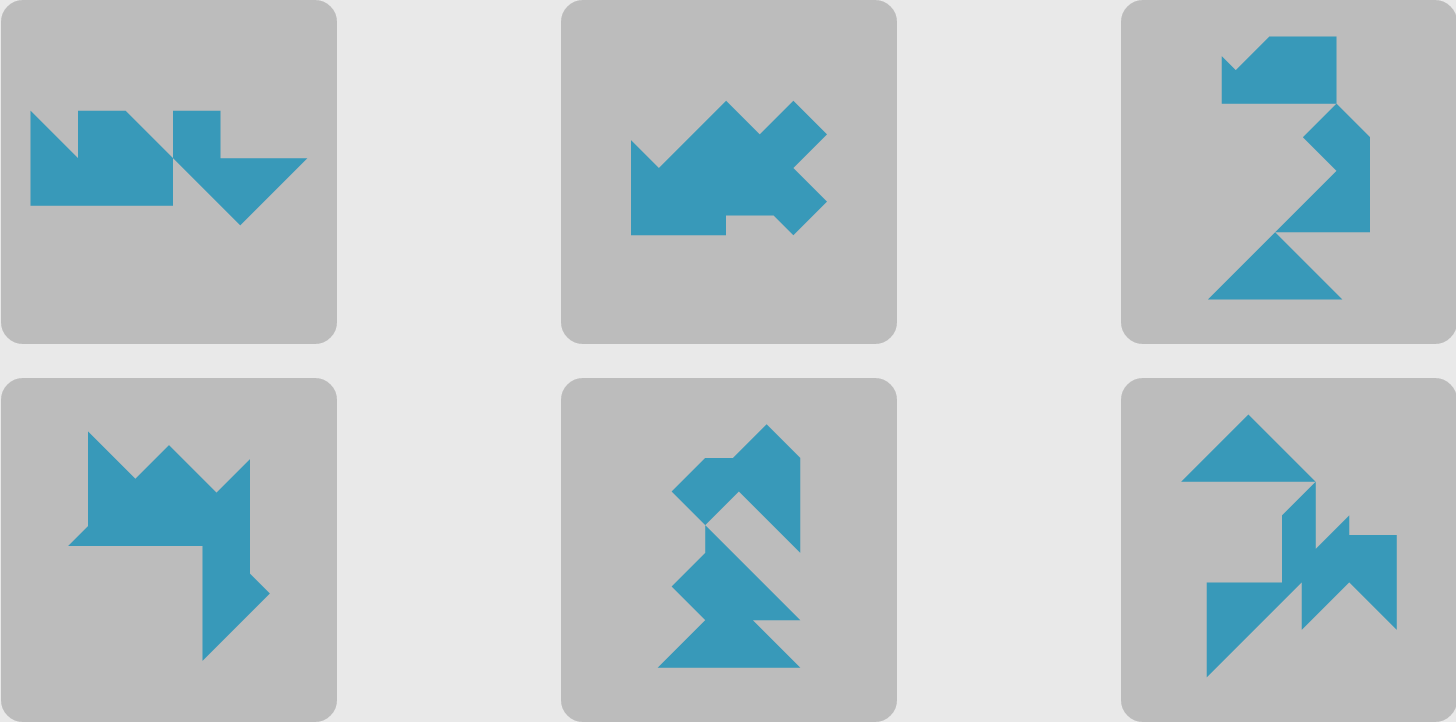
\includegraphics[width=0.45\textwidth]{figures/edges.png}}
    \hfill
  \subfloat[Edge-matching approach with lower range threshold]{\label{figur:4}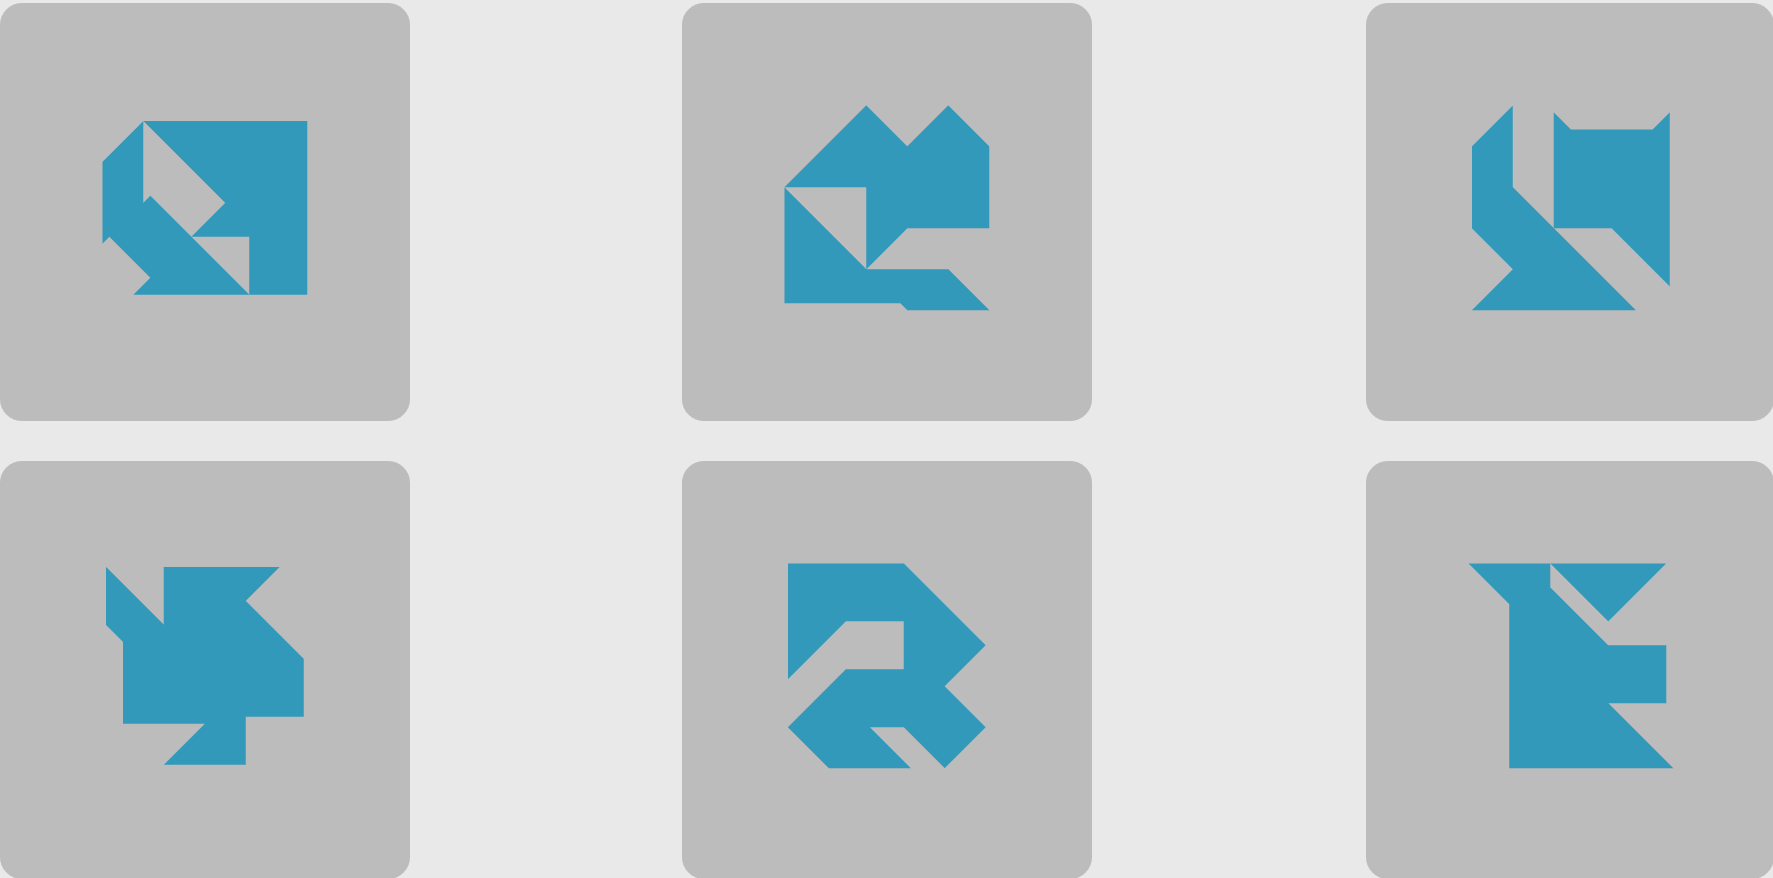
\includegraphics[width=0.45\textwidth]{figures/edgesSR.png}}
  \\
  \subfloat[Edge-matching approach with higher edge-matching weight]{\label{figur:5}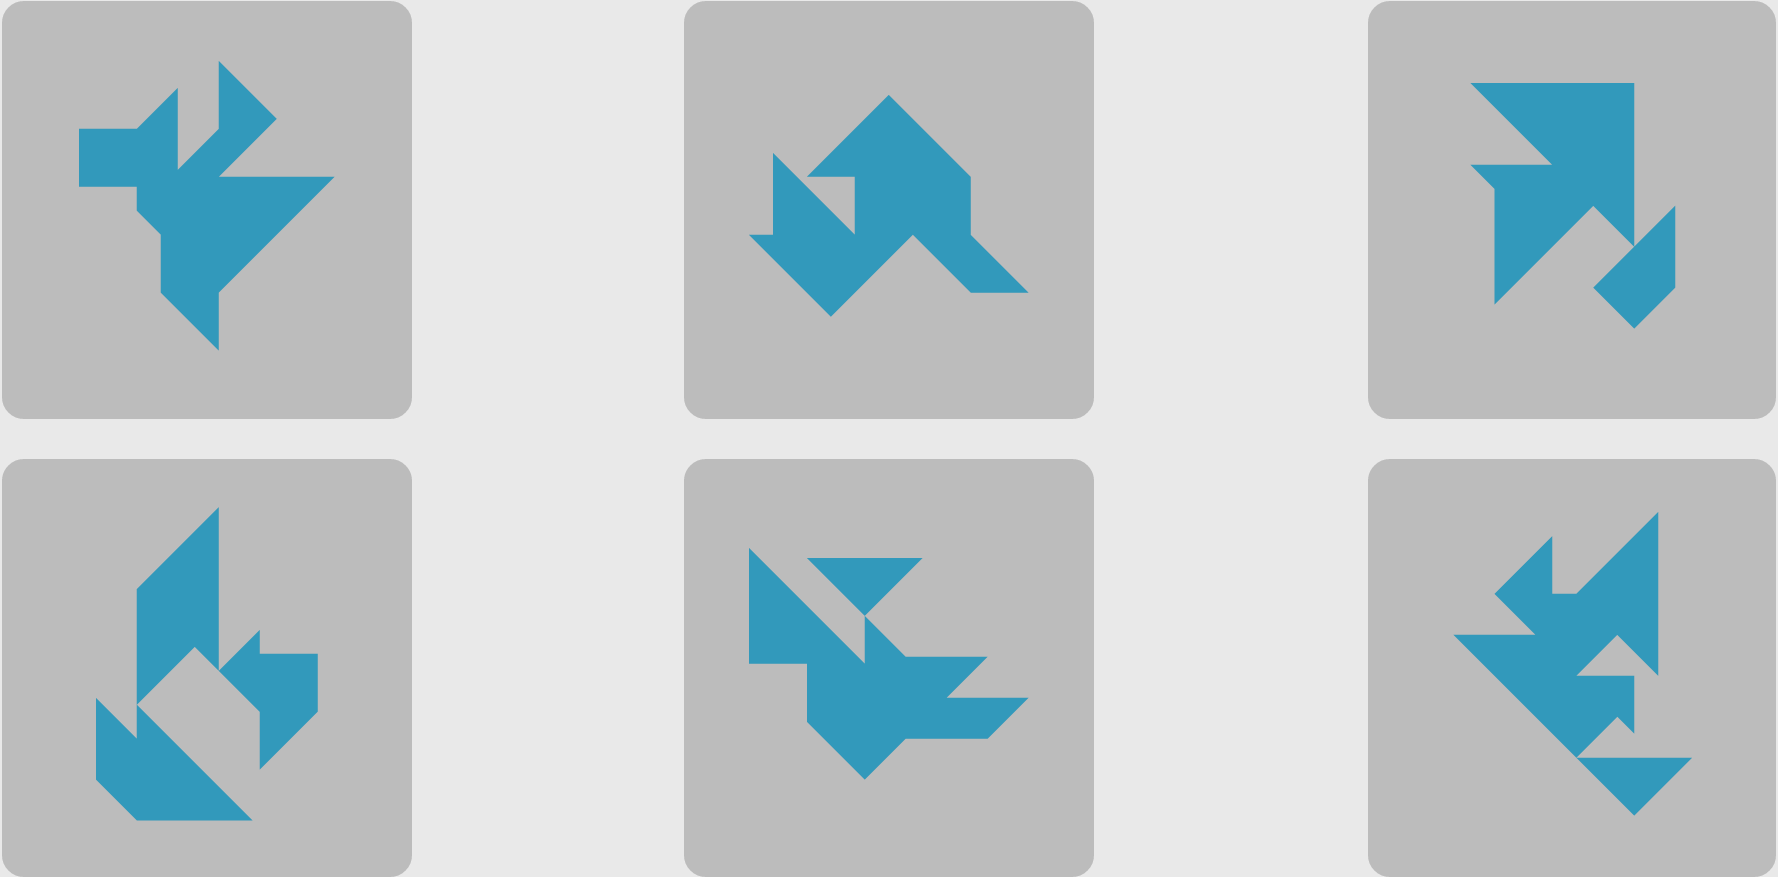
\includegraphics[width=0.45\textwidth]{figures/edgesLW.png}}
    \hfill
  \subfloat[Edge-matching approach with lower edge-matching weight]{\label{figur:6}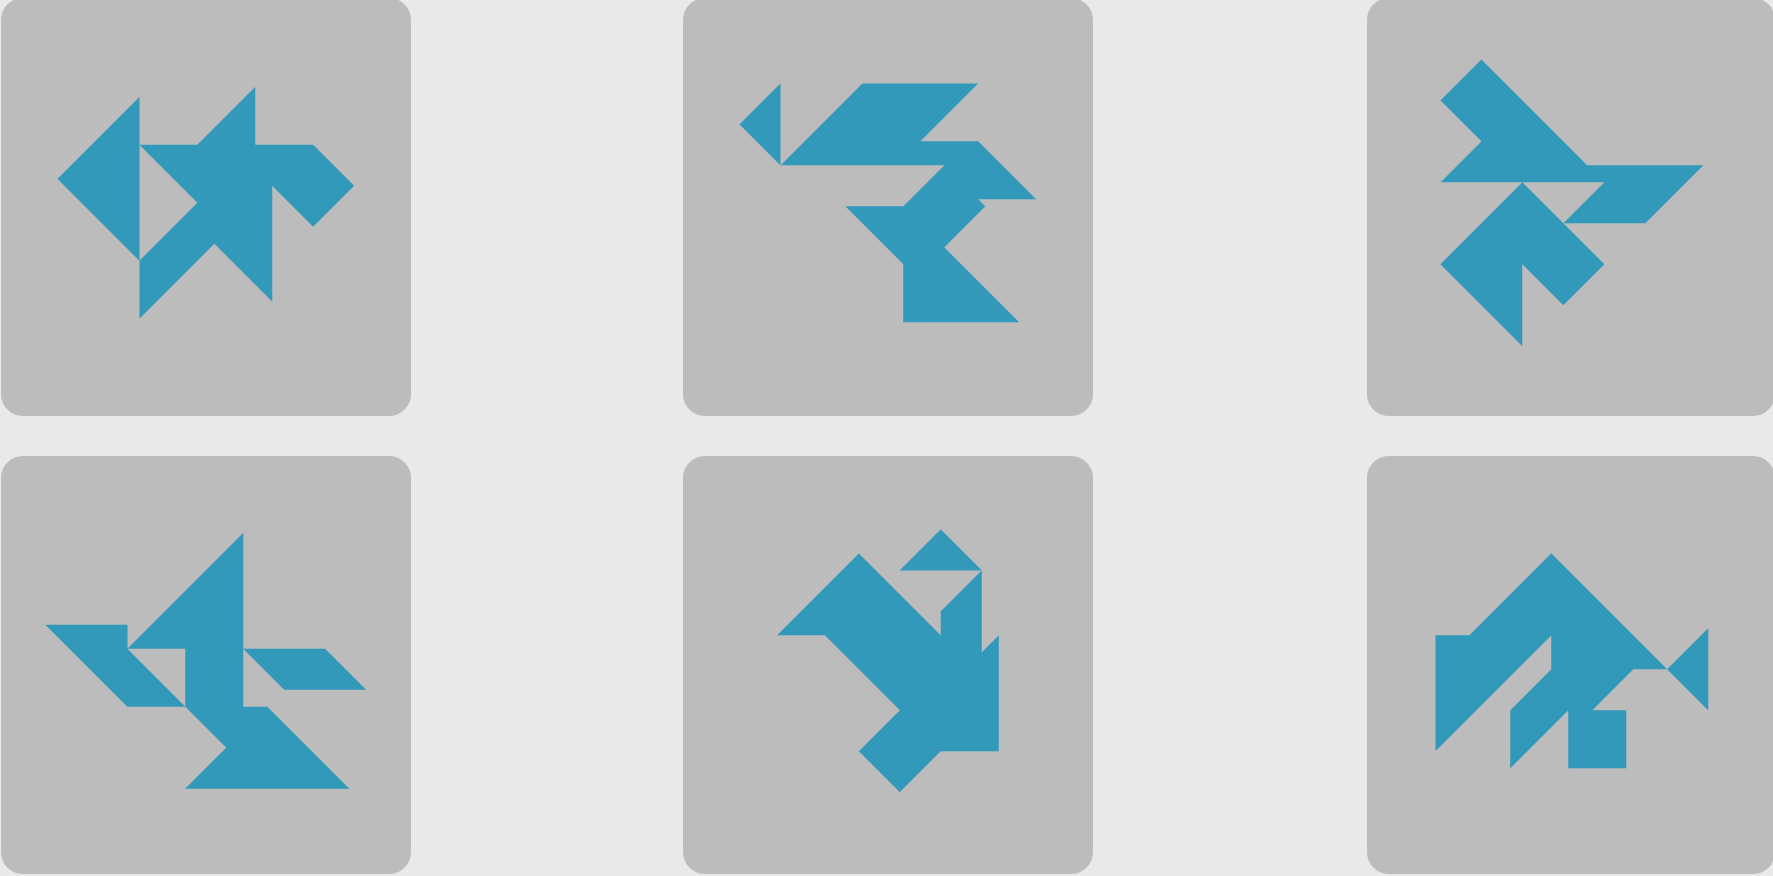
\includegraphics[width=0.45\textwidth]{figures/edgesSW}}
\caption{Results of generating six tangrams with different algorithms and different parameter settings}
\label{eval1}
\end{figure}